\documentclass[11pt,a4paper]{article}

\usepackage[margin=2.2cm]{geometry}
\usepackage[T1]{fontenc}
\usepackage[utf8]{inputenc}
\usepackage{lmodern}
\usepackage{microtype}
\usepackage{xcolor}
\usepackage{booktabs}
\usepackage{tabularx}
\usepackage{longtable}
\usepackage{enumitem}
\usepackage{float}
\usepackage{caption}
\usepackage{fancyhdr}
\usepackage{titlesec}
\usepackage{listings}
\usepackage{tikz}
\usetikzlibrary{arrows.meta,positioning,shapes.geometric,shapes.multipart,fit,backgrounds,calc}
\usepackage[hidelinks]{hyperref}

\definecolor{accent}{HTML}{2F6FDB}
\definecolor{codebg}{HTML}{F5F7FA}
\definecolor{boxfe}{HTML}{E8F0FE}
\definecolor{boxbe}{HTML}{E6F4EA}
\definecolor{boxml}{HTML}{FEF3E0}
\definecolor{boxdb}{HTML}{F3E8FD}

\hypersetup{colorlinks=true,linkcolor=accent,urlcolor=accent}
\titleformat{\section}{\Large\bfseries\color{accent}}{\thesection}{0.8em}{}
\titleformat{\subsection}{\large\bfseries}{\thesubsection}{0.8em}{}

\pagestyle{fancy}
\fancyhf{}
\lhead{Real-time Speech-to-Text}
\rhead{Technical Documentation}
\cfoot{\thepage}

\lstdefinestyle{code}{
  backgroundcolor=\color{codebg}, basicstyle=\ttfamily\small, breaklines=true,
  frame=single, rulecolor=\color{black!15}, keywordstyle=\color{accent}\bfseries,
  commentstyle=\color{black!55}\itshape, stringstyle=\color{teal!70!black},
  columns=fullflexible, keepspaces=true, xleftmargin=4pt, xrightmargin=4pt
}
\lstset{style=code}
\lstdefinelanguage{json}{
  morestring=[b]", literate={:}{{\textcolor{black!60}{:}}}1
}

\tikzset{
  box/.style={draw, rounded corners=3pt, align=center, minimum height=1.0cm, minimum width=2.9cm, font=\small},
  db/.style={draw, cylinder, shape border rotate=90, aspect=0.25, align=center, minimum height=1.3cm, minimum width=2.4cm, font=\small},
  arr/.style={-{Stealth[length=2.2mm]}, thick},
  lbl/.style={font=\scriptsize, fill=white, inner sep=1pt}
}

\title{\textbf{Real-time Speech-to-Text Service}\\[4pt]
\large Hindi $\cdot$ English $\cdot$ Hinglish transcription with a CRUD dashboard\\[2pt]
\normalsize Technical Documentation}
\author{Kasinadh Sarma}
\date{October 2026}

\begin{document}
\maketitle
\thispagestyle{empty}

\begin{center}
\begin{tabular}{@{}ll@{}}
\textbf{Live application} & \url{https://kasinadhsarma-speech-to-text.hf.space}\\
\textbf{Source code} & \url{https://github.com/kasinadhsarma/procucev-speech-to-text}\\
\textbf{Stack} & Python 3.12, FastAPI, WebSockets, SQLAlchemy, PostgreSQL, faster-whisper
\end{tabular}
\end{center}

\tableofcontents
\newpage

%--------------------------------------------------------------------
\section{Overview}
The service transcribes speech from the browser microphone \emph{as the user speaks}. Speech may mix
Hindi and English within one sentence. Each session is stored in a relational database, and a
dashboard provides create, read, update, delete and search over the transcription history.

\subsection*{Requirements met}
\begin{itemize}[leftmargin=*]
  \item \textbf{Real-time transcription:} partial text roughly every 1.5\,s, finalised at pauses.
  \item \textbf{Multilingual:} Whisper with automatic language detection and a Hinglish decoder prompt.
  \item \textbf{Self-hosted open-source STT:} OpenAI Whisper weights run through faster-whisper; no third-party speech API.
  \item \textbf{Relational database:} PostgreSQL (Neon) in production, SQLite fallback for local runs.
  \item \textbf{Dashboard with CRUD:} history list, search, create, edit and delete.
  \item \textbf{Deployed on the cloud:} Hugging Face Spaces, served over HTTPS/WSS.
\end{itemize}

%--------------------------------------------------------------------
\section{System Architecture}

\subsection{Component diagram}
\begin{figure}[H]
\centering
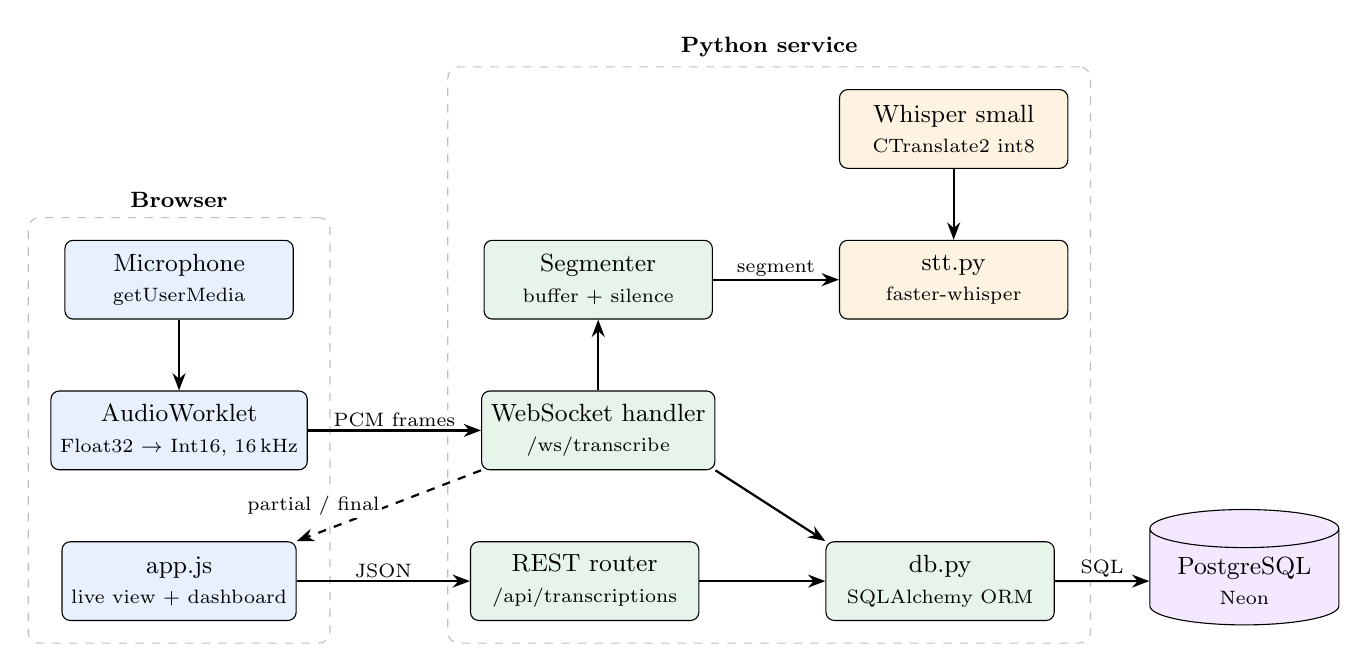
\begin{tikzpicture}[node distance=0.9cm and 1.1cm]
  \node[box, fill=boxfe] (mic) {Microphone\\\scriptsize getUserMedia};
  \node[box, fill=boxfe, below=of mic] (wk) {AudioWorklet\\\scriptsize Float32 $\to$ Int16, 16\,kHz};
  \node[box, fill=boxfe, below=of wk] (ui) {app.js\\\scriptsize live view + dashboard};

  \node[box, fill=boxbe, right=2.2cm of wk] (ws) {WebSocket handler\\\scriptsize /ws/transcribe};
  \node[box, fill=boxbe, right=2.2cm of ui] (rest) {REST router\\\scriptsize /api/transcriptions};
  \node[box, fill=boxbe, above=of ws] (seg) {Segmenter\\\scriptsize buffer + silence};

  \node[box, fill=boxml, right=1.6cm of seg] (stt) {stt.py\\\scriptsize faster-whisper};
  \node[box, fill=boxml, above=of stt] (model) {Whisper small\\\scriptsize CTranslate2 int8};
  \node[box, fill=boxbe, right=1.6cm of rest] (orm) {db.py\\\scriptsize SQLAlchemy ORM};
  \node[db, fill=boxdb, right=1.2cm of orm] (pg) {PostgreSQL\\\scriptsize Neon};

  \draw[arr] (mic) -- (wk);
  \draw[arr] (wk) -- node[lbl, above]{PCM frames} (ws);
  \draw[arr] (ws) -- (seg);
  \draw[arr] (seg) -- node[lbl, above]{segment} (stt);
  \draw[arr] (model) -- (stt);
  \draw[arr] (ws.south east) -- (orm.north west);
  \draw[arr, dashed] (ws.south west) -- node[lbl, left, xshift=-2pt]{partial / final} (ui.north east);
  \draw[arr] (ui) -- node[lbl, above]{JSON} (rest);
  \draw[arr] (rest) -- (orm);
  \draw[arr] (orm) -- node[lbl, above]{SQL} (pg);

  \begin{scope}[on background layer]
    \node[draw=black!25, dashed, rounded corners, fit=(mic)(wk)(ui), inner sep=8pt, label={[font=\footnotesize\bfseries]above:Browser}] {};
    \node[draw=black!25, dashed, rounded corners, fit=(seg)(ws)(rest)(stt)(model)(orm), inner sep=8pt, label={[font=\footnotesize\bfseries]above:Python service}] {};
  \end{scope}
\end{tikzpicture}
\caption{Main components and data flow.}
\end{figure}

\begin{table}[H]
\centering
\begin{tabularx}{\linewidth}{@{}lX@{}}
\toprule
\textbf{Module} & \textbf{Responsibility}\\
\midrule
\texttt{static/app.js} & Microphone capture, WebSocket streaming, live transcript rendering, dashboard CRUD\\
\texttt{app/main.py} & FastAPI application: REST endpoints, WebSocket endpoint, segmentation loop, static hosting\\
\texttt{app/stt.py} & Lazily loads one shared Whisper model; \texttt{transcribe(audio, language)}\\
\texttt{app/db.py} & Engine and session setup, \texttt{Transcription} ORM model, \texttt{DATABASE\_URL} normalisation\\
\texttt{hf\_entry.py} & Hugging Face entry point: Gradio owns port 7860; FastAPI routes are injected ahead of Gradio's\\
\bottomrule
\end{tabularx}
\caption{Source modules.}
\end{table}

\subsection{Real-time sequence}
\begin{figure}[H]
\centering
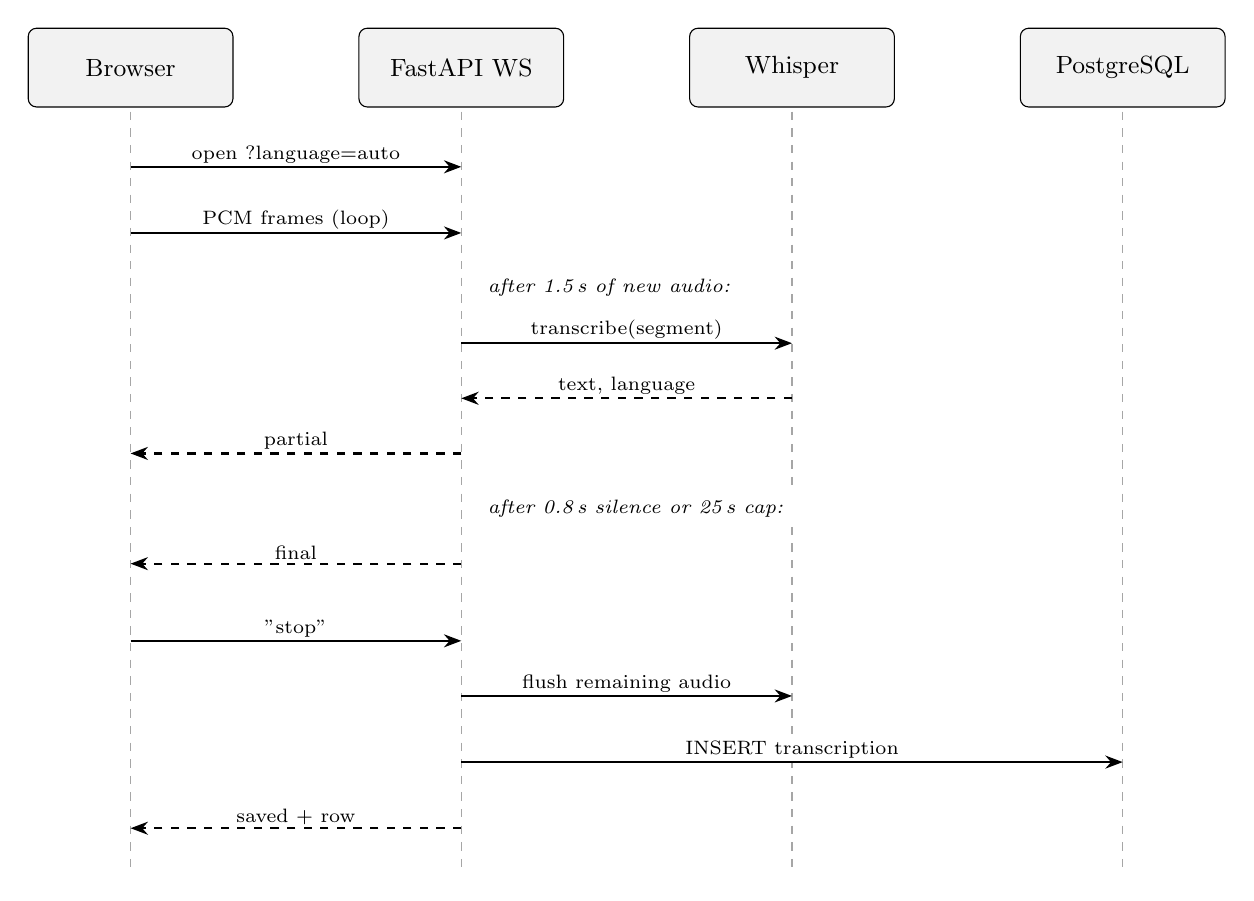
\begin{tikzpicture}[x=4.2cm, y=-0.7cm, font=\small]
  \foreach \x/\name in {0/Browser, 1/FastAPI WS, 2/Whisper, 3/PostgreSQL} {
    \node[box, minimum width=2.6cm, fill=black!5] at (\x,0) {\name};
    \draw[black!35, dashed] (\x,0.8) -- (\x,14.6);
  }
  \newcommand{\msg}[4]{\draw[arr] (#1,#3) -- node[lbl, above]{#4} (#2,#3);}
  \newcommand{\ret}[4]{\draw[arr, dashed] (#1,#3) -- node[lbl, above]{#4} (#2,#3);}
  \msg{0}{1}{1.8}{open ?language=auto}
  \msg{0}{1}{3.0}{PCM frames (loop)}
  \node[font=\scriptsize\itshape, anchor=west, fill=white] at (1.05,4.0) {after 1.5\,s of new audio:};
  \msg{1}{2}{5.0}{transcribe(segment)}
  \ret{2}{1}{6.0}{text, language}
  \ret{1}{0}{7.0}{partial}
  \node[font=\scriptsize\itshape, anchor=west, fill=white] at (1.05,8.0) {after 0.8\,s silence or 25\,s cap:};
  \ret{1}{0}{9.0}{final}
  \msg{0}{1}{10.4}{"stop"}
  \msg{1}{2}{11.4}{flush remaining audio}
  \msg{1}{3}{12.6}{INSERT transcription}
  \ret{1}{0}{13.8}{saved + row}
\end{tikzpicture}
\caption{Streaming transcription over one WebSocket session.}
\end{figure}

\subsection{Segmentation algorithm}
Whisper is not a streaming model, so the server keeps a growing \emph{segment} buffer and re-decodes it:
\begin{enumerate}[leftmargin=*]
  \item Append each incoming Int16 frame (scaled to Float32 in $[-1,1]$) to the segment buffer.
  \item If the last 0.8\,s has RMS energy $< 0.012$ and the segment is longer than 1\,s, or the segment
        exceeds 25\,s: decode it, send a \texttt{final} message and clear the buffer.
  \item Otherwise, if 1.5\,s of new audio arrived since the last decode: decode and send a \texttt{partial} message.
  \item On \texttt{stop}: decode what remains, join all finals, store one row and send \texttt{saved}.
\end{enumerate}
Decoding runs in a worker thread (\texttt{asyncio.to\_thread}) so the event loop keeps receiving audio.

\begin{table}[H]
\centering
\begin{tabular}{@{}lll@{}}
\toprule
\textbf{Parameter} & \textbf{Value} & \textbf{Constant}\\
\midrule
Sample format & 16\,000\,Hz, mono, Int16 LE & \texttt{SAMPLE\_RATE}\\
Partial interval & 1.5\,s & \texttt{PARTIAL\_EVERY\_SEC}\\
Silence window / threshold & 0.8\,s / RMS 0.012 & \texttt{SILENCE\_SEC}, \texttt{SILENCE\_RMS}\\
Maximum segment & 25\,s & \texttt{MAX\_SEGMENT\_SEC}\\
Decoder & beam 1, VAD filter, Hinglish prompt & \texttt{stt.transcribe}\\
\bottomrule
\end{tabular}
\caption{Real-time tuning parameters.}
\end{table}

%--------------------------------------------------------------------
\section{Database Design}

\subsection{Entity}
\begin{figure}[H]
\centering
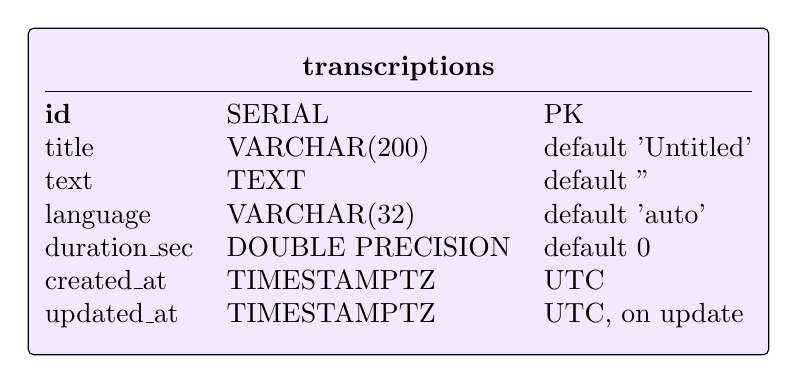
\begin{tikzpicture}
  \node[draw, fill=boxdb, rounded corners=2pt, inner sep=6pt] (t) {
    \begin{tabular}{@{}l@{\hspace{1.2em}}l@{\hspace{1.2em}}l@{}}
      \multicolumn{3}{c}{\rule{0pt}{2.6ex}\textbf{transcriptions}}\\[2pt]\hline
      \rule{0pt}{2.6ex}\textbf{id} & SERIAL & PK\\
      title & VARCHAR(200) & default 'Untitled'\\
      text & TEXT & default ''\\
      language & VARCHAR(32) & default 'auto'\\
      duration\_sec & DOUBLE PRECISION & default 0\\
      created\_at & TIMESTAMPTZ & UTC\\
      updated\_at & TIMESTAMPTZ & UTC, on update\\[2pt]
    \end{tabular}};
\end{tikzpicture}
\caption{Table \texttt{transcriptions}.}
\end{figure}

\subsection{DDL}
\begin{lstlisting}[language=SQL]
CREATE TABLE transcriptions (
    id            SERIAL PRIMARY KEY,
    title         VARCHAR(200)      NOT NULL DEFAULT 'Untitled',
    text          TEXT              NOT NULL DEFAULT '',
    language      VARCHAR(32)       NOT NULL DEFAULT 'auto',
    duration_sec  DOUBLE PRECISION  NOT NULL DEFAULT 0,
    created_at    TIMESTAMPTZ       NOT NULL DEFAULT now(),
    updated_at    TIMESTAMPTZ       NOT NULL DEFAULT now()
);
\end{lstlisting}
Defaults are applied by the SQLAlchemy model; the table is created on startup by
\texttt{Base.metadata.create\_all()}.

\subsection{Queries}
\begin{table}[H]
\centering
\begin{tabularx}{\linewidth}{@{}lX@{}}
\toprule
\textbf{Operation} & \textbf{SQL (simplified)}\\
\midrule
List & \texttt{SELECT * FROM transcriptions ORDER BY created\_at DESC, id DESC LIMIT :limit OFFSET :offset}\\
Search & \texttt{... WHERE text ILIKE :p OR title ILIKE :p}\\
Read & \texttt{SELECT * FROM transcriptions WHERE id = :id}\\
Create & \texttt{INSERT INTO transcriptions (...) VALUES (...) RETURNING id}\\
Update & \texttt{UPDATE transcriptions SET ..., updated\_at = :now WHERE id = :id}\\
Delete & \texttt{DELETE FROM transcriptions WHERE id = :id}\\
\bottomrule
\end{tabularx}
\end{table}

\subsection{Connection handling}
\texttt{DATABASE\_URL} selects the backend (unset means SQLite). Before connecting, \texttt{app/db.py}
strips whitespace and quotes, rewrites \texttt{postgres://} and \texttt{postgresql://} to
\texttt{postgresql+psycopg2://}, removes Neon's \texttt{channel\_binding=require}
(TLS is still enforced by \texttt{sslmode=require}), and enables \texttt{pool\_pre\_ping}.
\texttt{GET /api/health} reports the active backend.

%--------------------------------------------------------------------
\section{API Specification}

\subsection{REST endpoints}
\begin{table}[H]
\centering
\begin{tabularx}{\linewidth}{@{}llXl@{}}
\toprule
\textbf{Method} & \textbf{Path} & \textbf{Description} & \textbf{Success}\\
\midrule
GET & \texttt{/api/health} & Liveness, model, database backend & 200\\
GET & \texttt{/api/transcriptions} & List; \texttt{q}, \texttt{limit} (1--200), \texttt{offset} & 200\\
POST & \texttt{/api/transcriptions} & Create & 201\\
GET & \texttt{/api/transcriptions/\{id\}} & Read one & 200 / 404\\
PUT & \texttt{/api/transcriptions/\{id\}} & Partial update & 200 / 404\\
DELETE & \texttt{/api/transcriptions/\{id\}} & Delete & 204 / 404\\
\bottomrule
\end{tabularx}
\end{table}

\subsection{Transcription schema}
\begin{lstlisting}[language=json]
{
  "id": 1,
  "title": "Kal subah meeting hai...",
  "text": "Kal subah meeting hai, please slides ready rakhna.",
  "language": "hi",
  "duration_sec": 4.12,
  "created_at": "2026-10-22T11:40:02.118Z",
  "updated_at": "2026-10-22T11:40:02.118Z"
}
\end{lstlisting}
Create body: \texttt{title} (max 200, default \texttt{"Untitled"}), \texttt{text}, \texttt{language}
(default \texttt{"auto"}), \texttt{duration\_sec}. Update body: any subset of \texttt{title},
\texttt{text}, \texttt{language}. Errors return \texttt{\{"detail": "..."\}}; validation errors return 422.

\subsection{WebSocket protocol}
Endpoint: \texttt{wss://<host>/ws/transcribe?language=auto|hi|en}.

\begin{table}[H]
\centering
\begin{tabularx}{\linewidth}{@{}llX@{}}
\toprule
\textbf{Direction} & \textbf{Frame} & \textbf{Meaning}\\
\midrule
client $\to$ server & binary & Int16 LE PCM, mono, 16\,kHz, any chunk size\\
client $\to$ server & text \texttt{stop} & Flush, save and close\\
server $\to$ client & \texttt{\{"type":"partial","text","language"\}} & Provisional text, may change\\
server $\to$ client & \texttt{\{"type":"final","text","language"\}} & Stable text for a closed segment\\
server $\to$ client & \texttt{\{"type":"saved","transcription"\}} & Stored row, or \texttt{null} if nothing recognised\\
server $\to$ client & \texttt{\{"type":"error","message"\}} & Unexpected server error\\
\bottomrule
\end{tabularx}
\end{table}

%--------------------------------------------------------------------
\section{Technology Stack}
\begin{longtable}{@{}p{3.4cm}p{1.6cm}p{2.4cm}p{7.2cm}@{}}
\toprule
\textbf{Library} & \textbf{Version} & \textbf{License} & \textbf{Purpose}\\
\midrule
\endhead
FastAPI & 0.159 & MIT & REST and WebSocket endpoints, OpenAPI docs\\
Starlette & 1.9 & BSD-3-Clause & ASGI toolkit, static files, WebSockets\\
Uvicorn & 0.54 & BSD-3-Clause & ASGI server\\
Pydantic & 2.14 & MIT & Request validation\\
SQLAlchemy & 2.1 & MIT & ORM and database engine\\
psycopg2-binary & 2.9 & LGPL-3.0 & PostgreSQL driver\\
faster-whisper & 1.2 & MIT & Whisper inference with VAD filter\\
CTranslate2 & 4.8 & MIT & Optimised int8 CPU inference\\
NumPy & 2.x & BSD-3-Clause & PCM buffers and RMS silence detection\\
Whisper \emph{small} & -- & MIT & 244\,M-parameter multilingual ASR model\\
Gradio & 6.x & Apache-2.0 & HTTP host on Hugging Face ZeroGPU\\
pytest, HTTPX & -- & MIT, BSD-3 & Tests\\
websockets & 17.x & BSD-3-Clause & Streaming test client\\
PostgreSQL (Neon) & 16 & PostgreSQL & Production database\\
\bottomrule
\end{longtable}

Frontend: HTML5, CSS3 and vanilla JavaScript using \texttt{getUserMedia}, \texttt{AudioContext},
\texttt{AudioWorklet}, \texttt{WebSocket}, \texttt{fetch} and \texttt{<dialog>}. There is no build step.

%--------------------------------------------------------------------
\section{Deployment}

\begin{figure}[H]
\centering
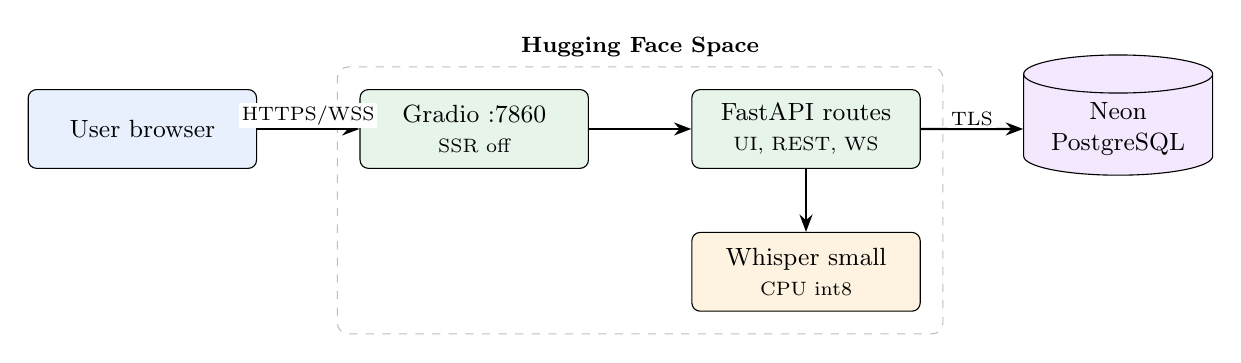
\begin{tikzpicture}[node distance=0.8cm and 1.3cm]
  \node[box, fill=boxfe] (user) {User browser};
  \node[box, fill=boxbe, right=of user] (gr) {Gradio :7860\\\scriptsize SSR off};
  \node[box, fill=boxbe, right=of gr] (fa) {FastAPI routes\\\scriptsize UI, REST, WS};
  \node[box, fill=boxml, below=of fa] (wh) {Whisper small\\\scriptsize CPU int8};
  \node[db, fill=boxdb, right=of fa] (neon) {Neon\\PostgreSQL};
  \draw[arr] (user) -- node[lbl, above]{HTTPS/WSS} (gr);
  \draw[arr] (gr) -- (fa);
  \draw[arr] (fa) -- (wh);
  \draw[arr] (fa) -- node[lbl, above]{TLS} (neon);
  \begin{scope}[on background layer]
    \node[draw=black!25, dashed, rounded corners, fit=(gr)(fa)(wh), inner sep=8pt, label={[font=\footnotesize\bfseries]above:Hugging Face Space}] {};
  \end{scope}
\end{tikzpicture}
\caption{Production deployment.}
\end{figure}

\subsection{Hugging Face Spaces}
Free accounts get ZeroGPU hardware for Gradio-SDK Spaces, which only starts if Gradio launches an app
containing an \texttt{@spaces.GPU} function. \texttt{hf\_entry.py} therefore lets Gradio own port 7860
with a hidden placeholder function and passes the FastAPI routes through \texttt{app\_kwargs}, so they
take precedence. Server-side rendering is disabled because its Node proxy would hide those routes.
Transcription runs on CPU. The Neon connection string is stored as the Space secret \texttt{DATABASE\_URL}.

\subsection{Local and container options}
\begin{lstlisting}[language=bash]
# Full stack with PostgreSQL
docker compose up --build              # http://localhost:8000

# Without Docker (SQLite)
python3 -m venv .venv && .venv/bin/pip install -r requirements.txt
.venv/bin/uvicorn app.main:app

# Tests
.venv/bin/pip install -r requirements-dev.txt && .venv/bin/pytest -q
\end{lstlisting}

\subsection{Configuration}
\begin{table}[H]
\centering
\begin{tabularx}{\linewidth}{@{}llX@{}}
\toprule
\textbf{Variable} & \textbf{Default} & \textbf{Description}\\
\midrule
\texttt{DATABASE\_URL} & SQLite file & SQLAlchemy URL\\
\texttt{WHISPER\_MODEL} & \texttt{small} & \texttt{tiny}, \texttt{base}, \texttt{small}, \texttt{medium}, \texttt{large-v3}\\
\texttt{WHISPER\_DEVICE} & \texttt{cpu} & \texttt{cpu} or \texttt{cuda}\\
\texttt{WHISPER\_COMPUTE} & \texttt{int8} & CTranslate2 compute type\\
\texttt{WHISPER\_THREADS} & 4 & Inference CPU threads\\
\texttt{WHISPER\_PROMPT} & Hinglish sentence & Decoder initial prompt\\
\texttt{PRELOAD\_MODEL} & 1 & Load model at startup\\
\texttt{PORT} & 7860 & HTTP port\\
\bottomrule
\end{tabularx}
\end{table}

%--------------------------------------------------------------------
\section{Code Reference}
Every module, attribute, class and function. The source docstrings match this section.

\subsection{Class diagram}
\begin{figure}[H]
\centering
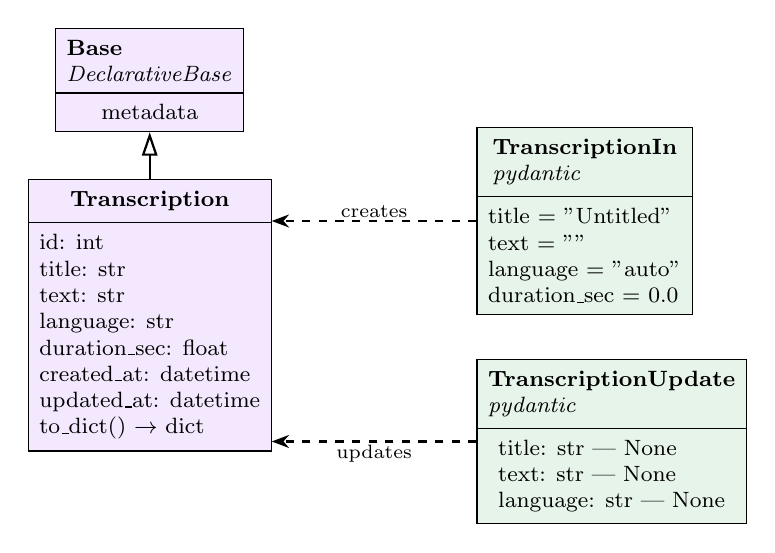
\begin{tikzpicture}[font=\small, node distance=0.6cm and 2.6cm]
  \tikzset{cls/.style={draw, rectangle split, rectangle split parts=2, align=left, fill=#1, inner sep=4pt, font=\footnotesize}}
  \node[cls=boxdb] (base) {\textbf{Base}\\\textit{DeclarativeBase}\nodepart{second}metadata};
  \node[cls=boxdb, below=of base] (tr) {\textbf{Transcription}\nodepart{second}id: int\\title: str\\text: str\\language: str\\duration\_sec: float\\created\_at: datetime\\updated\_at: datetime\\\rule{0pt}{2ex}to\_dict() $\to$ dict};
  \node[cls=boxbe, right=of tr, yshift=1.2cm] (tin) {\textbf{TranscriptionIn}\\\textit{pydantic}\nodepart{second}title = "Untitled"\\text = ""\\language = "auto"\\duration\_sec = 0.0};
  \node[cls=boxbe, right=of tr, yshift=-1.6cm] (tup) {\textbf{TranscriptionUpdate}\\\textit{pydantic}\nodepart{second}title: str | None\\text: str | None\\language: str | None};
  \draw[-{Triangle[open,length=3mm]}, thick] (tr) -- (base);
  \draw[arr, dashed] (tin.west) -- node[lbl, above]{creates} (tr.east |- tin.west);
  \draw[arr, dashed] (tup.west) -- node[lbl, below]{updates} (tr.east |- tup.west);
\end{tikzpicture}
\caption{Data classes.}
\end{figure}

\subsection{\texttt{app/db.py}}
\begin{longtable}{@{}p{4.6cm}p{10.6cm}@{}}
\toprule
\textbf{Name} & \textbf{Description}\\
\midrule
\endhead
\texttt{DATABASE\_URL} & \texttt{\$DATABASE\_URL} or \texttt{sqlite:///./transcriptions.db}; stripped of whitespace/quotes, driver set to \texttt{postgresql+psycopg2}, \texttt{channel\_binding=require} removed\\
\texttt{connect\_args} & \texttt{\{"check\_same\_thread": False\}} for SQLite, otherwise empty\\
\texttt{engine} & \texttt{create\_engine(DATABASE\_URL, pool\_pre\_ping=True)}\\
\texttt{SessionLocal} & \texttt{sessionmaker(bind=engine, expire\_on\_commit=False)}\\
\texttt{utcnow()} & Returns \texttt{datetime.now(timezone.utc)}; timestamp default and \texttt{onupdate}\\
\texttt{Base} & SQLAlchemy \texttt{DeclarativeBase}\\
\texttt{Transcription} & ORM model for \texttt{transcriptions}; attributes in Section 3\\
\texttt{to\_dict()} & Method of \texttt{Transcription}: JSON-ready dict; duration rounded to 0.01\,s, ISO 8601 timestamps\\
\texttt{init\_db()} & \texttt{Base.metadata.create\_all(engine)}; idempotent\\
\bottomrule
\end{longtable}

\subsection{\texttt{app/stt.py}}
\begin{longtable}{@{}p{4.6cm}p{10.6cm}@{}}
\toprule
\textbf{Name} & \textbf{Description}\\
\midrule
\endhead
\texttt{SAMPLE\_RATE} & 16000\\
\texttt{MODEL\_SIZE} & \texttt{\$WHISPER\_MODEL}, default \texttt{small}\\
\texttt{HINGLISH\_PROMPT} & \texttt{\$WHISPER\_PROMPT}, default Hinglish sentence; decoder \texttt{initial\_prompt}\\
\texttt{\_model}, \texttt{\_lock} & Shared \texttt{WhisperModel} (lazy) and the lock guarding its creation\\
\texttt{get\_model()} & Thread-safe lazy load: \texttt{WhisperModel(MODEL\_SIZE, device, compute\_type, cpu\_threads)} from \texttt{WHISPER\_DEVICE}/\texttt{COMPUTE}/\texttt{THREADS}. First call downloads weights.\\
\texttt{transcribe()} & \texttt{transcribe(audio, language=None)}. \textbf{Args:} float32 mono 16\,kHz array in $[-1,1]$; language code or \texttt{auto}. \textbf{Returns} \texttt{(text, language)}. Skips audio under 0.3\,s. Decodes with \texttt{beam\_size=1}, \texttt{vad\_filter=True}, \texttt{condition\_on\_previous\_text=False}.\\
\bottomrule
\end{longtable}

\subsection{\texttt{app/main.py}}
\begin{longtable}{@{}p{4.6cm}p{10.6cm}@{}}
\toprule
\textbf{Name} & \textbf{Description}\\
\midrule
\endhead
\texttt{STATIC} & Path of the \texttt{static/} directory\\
\texttt{PARTIAL\_EVERY\_SEC} & 1.5 --- new audio between partial decodes\\
\texttt{SILENCE\_SEC} & 0.8\,s trailing window checked for silence\\
\texttt{SILENCE\_RMS} & 0.012 RMS threshold\\
\texttt{MAX\_SEGMENT\_SEC} & 25.0 --- forces a final decode\\
\texttt{app} & \texttt{FastAPI(title="Speech to Text", lifespan=lifespan)}\\
\texttt{lifespan(\_)} & Startup: \texttt{init\_db()}; loads the model in a thread unless \texttt{PRELOAD\_MODEL=0}\\
\texttt{get\_db()} & Dependency yielding a session, closed in \texttt{finally}\\
\texttt{TranscriptionIn} & \texttt{title} (max 200, "Untitled"), \texttt{text} (""), \texttt{language} ("auto"), \texttt{duration\_sec} (0.0)\\
\texttt{TranscriptionUpdate} & Optional \texttt{title} (max 200), \texttt{text}, \texttt{language}\\
\texttt{health()} & \texttt{GET /api/health} $\to$ status, model, \texttt{engine.dialect.name}\\
\texttt{list\_transcriptions()} & \texttt{GET}; params \texttt{q}, \texttt{limit}, \texttt{offset}; newest first; \texttt{ILIKE} on title/text; \texttt{limit} 1--200\\
\texttt{create\_transcription()} & \texttt{POST}; body \texttt{TranscriptionIn}; \texttt{Transcription(**body.model\_dump())}; 201\\
\texttt{\_get\_or\_404()} & Args \texttt{db}, \texttt{tid}: \texttt{db.get(...)} or \texttt{HTTPException(404)}\\
\texttt{get\_transcription()} & \texttt{GET /\{tid\}}\\
\texttt{update\_transcription()} & \texttt{PUT /\{tid\}}, body \texttt{TranscriptionUpdate}; sets only provided non-null fields\\
\texttt{delete\_transcription()} & \texttt{DELETE /\{tid\}}; 204\\
\texttt{ws\_transcribe()} & Args \texttt{ws}, \texttt{language}. WebSocket loop (Section 2.3). State: \texttt{segment}, \texttt{since\_decode}, \texttt{finals}, \texttt{langs}, \texttt{total\_samples}. Saves one row on stop.\\
\quad\texttt{decode(final)} & Nested; transcribes \texttt{segment} in a thread, sends partial/final, clears the segment when final\\
\texttt{index()} & \texttt{GET /} $\to$ \texttt{static/index.html}\\
\bottomrule
\end{longtable}

\subsection{\texttt{hf\_entry.py}}
\begin{longtable}{@{}p{4.6cm}p{10.6cm}@{}}
\toprule
\textbf{Name} & \textbf{Description}\\
\midrule
\endhead
\texttt{\_quiet\_unraisable(u)} & Replaces \texttt{sys.unraisablehook}; ignores ``Invalid file descriptor'' errors from discarded event loops\\
\texttt{gpu} & \texttt{spaces.GPU}, or a no-op decorator locally\\
\texttt{\_placeholder(x)} & Identity function marked \texttt{@gpu} for ZeroGPU's startup check\\
\texttt{demo} & Hidden \texttt{gr.Blocks} app\\
\texttt{\_\_main\_\_} & \texttt{init\_db()}, warm model in a thread, \texttt{demo.launch(port 7860, ssr\_mode=False, app\_kwargs=\{"routes": stt\_app.routes\})}\\
\bottomrule
\end{longtable}

\subsection{\texttt{static/app.js}}
\begin{longtable}{@{}p{4.6cm}p{10.6cm}@{}}
\toprule
\textbf{Name} & \textbf{Description}\\
\midrule
\endhead
\texttt{\$}, \texttt{api}, \texttt{esc(s)} & Selector shorthand, API base path, HTML escaping\\
\texttt{editing}, \texttt{t} & Row being edited; search debounce timer\\
\texttt{ws}, \texttt{ctx}, \texttt{stream}, \texttt{node} & WebSocket, 16\,kHz \texttt{AudioContext}, microphone stream, worklet node\\
\texttt{recording}, \texttt{finals} & Capture flag; final segments this session\\
\texttt{load()} & Fetches and renders the history (with search)\\
\texttt{openDialog(row)} & Opens create/edit dialog\\
\texttt{renderLive(partial)} & Final text plus grey partial text\\
\texttt{start()} & Microphone $\to$ WebSocket $\to$ AudioWorklet streaming; handles \texttt{partial}/\texttt{final}/\texttt{saved}/\texttt{error}\\
\texttt{stop()}, \texttt{cleanup()} & Send \texttt{stop}; release microphone and audio graph\\
\texttt{PCM.process()} & Worklet: Float32 block $\to$ Int16, posted as a transferable buffer\\
Event handlers & \texttt{\#new}, \texttt{\#cancel}, \texttt{\#form} submit (POST/PUT), \texttt{\#list} (edit/delete), \texttt{\#search} (250\,ms debounce), \texttt{\#rec} (start/stop)\\
\bottomrule
\end{longtable}

%--------------------------------------------------------------------
\section{Testing}
\begin{itemize}[leftmargin=*]
  \item \textbf{Unit/API:} \texttt{tests/test\_api.py} exercises create, read, search, update, delete and 404 handling
        against a temporary SQLite database, with Hindi (Devanagari) text.
  \item \textbf{End-to-end streaming:} \texttt{tests/stream\_demo.py} streams a 16\,kHz PCM recording of a mixed
        Hindi/English sentence in real time, locally or against the live \texttt{wss://} endpoint, and prints
        the partial, final and saved messages.
\end{itemize}

%--------------------------------------------------------------------
\section{Limitations and Future Work}
\begin{itemize}[leftmargin=*]
  \item No authentication; all visitors share one history. Next: user accounts and a \texttt{user\_id} column.
  \item No migration tool; add Alembic.
  \item One shared model instance; concurrent sessions queue for CPU. Next: GPU inference or a worker pool.
  \item Accented English may be transliterated into Devanagari; larger models reduce this.
  \item Energy-based segmentation can mis-split in noisy rooms; a streaming VAD (e.g.\ Silero on the client) would help.
  \item Full-text search at scale: \texttt{pg\_trgm} GIN index.
\end{itemize}

\end{document}
